\documentclass[11pt,oneside,titlepage]{report}
\usepackage[T1]{fontenc}
%\usepackage[utf8]{inputenc}
%\usepackage[english,polish]{babel}
%\usepackage{polski}
\usepackage{graphicx}
\usepackage{subcaption}
\makeatletter
\usepackage[top=2cm, bottom=3cm, left=2cm, right=2cm]{geometry}
\usepackage{fancyhdr}

\author{Adam Cisowski}
\title{CFD calculations of Formula Student car in OpenFoam on AWS cluster}



\newcommand{\linia}{\rule{\linewidth}{0.4mm}}
\renewcommand{\maketitle}{\begin{titlepage}
    \vspace*{0cm}
    \begin{center}
    Politechnika Warszawska\\
    Wydzial Mechaniczny Energetyki i Lotnictwa\\
    
    
    \end{center}
    \vspace{3cm}
    \noindent\linia
    \begin{center}
      \LARGE \textsc{\@title}
         \end{center}
     \linia
	\vspace{1cm}     
     \begin{center}\large
     Obliczenia inżynierskie w chmurze
     \end{center}
    \vspace{2cm}
   
    \begin{center}\Large 
    \@author
    
    \end{center}
    \vspace{9cm}
    \begin{center}
    \@date
    \end{center}
  \end{titlepage}%
}
\makeatother

%\date{16 June 2018}



\renewcommand*\thesection{\arabic{section}} % zmiana numeracji sekcji 0.X -> X





\begin{document}
\pagestyle{fancy}
\rhead{czesc\\czesc\\czesc\\czesc}
\rhead{
\includegraphics[height=1cm]{pobrane.jpg}}
\lhead{}

\maketitle
\tableofcontents
\newpage




\section{Introduction}

Formula Student is a student engineering competition in which participate over 800 teams from around the world. WUT Racing Team from Warsaw University of Technology has taken part in the competitions from six years. Two constructions has been built and now third construction is being designed. Conception of aerodynamic package is to generate as big down force as it is possible irrespective of drag forces. It makes sens because of low maximum speed during the competitions (it is max 90kmph). The down force increase friction between road and tires. Thanks for that the car rides faster in turns.

In this report will be presented OpenFoam's calculations of entire Formula Student car in comparison to Ansys Fluent's calculations on the same mesh.  
\section{Model}
The model was created in Siemens NX. Each aerodynamic element has been optimized firstly in 2D, next in 3D. 


\begin{figure}[h!]
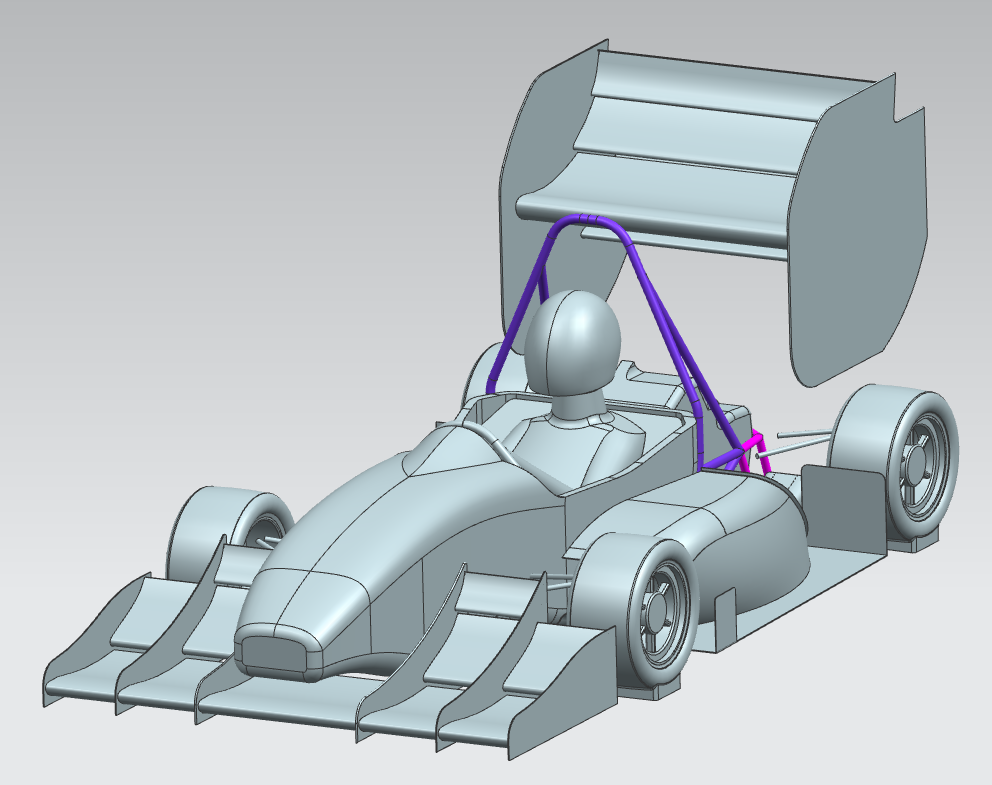
\includegraphics[width=\textwidth]{img/final}
\caption{WUT3 aerodynamics model}
%\label{fig:boat1}
\end{figure}



\section{Mesh}
The mesh was created in Ansys Mesher. It was very difficult to generate good quality mesh, because of complex geometry. Minimum Orthogonal Quality of the mesh is about 7e-02.

It is worth to mention that the mesh has to be export in ASCII format. OpenFoam is working on ASCII and it does not read the mesh wrote in binary. 

Firstly, the mesh was created with boundary layer, which improve calculations precision near walls. Unfortunately, quality of the mesh getting worse with boundary layer and OpenFoam could not calculate this. The residuals and forces reached large values. In this case Fluent was better than OpenFoam, because it made calculations and results was quite good.

In external flow calculations very good option is polyhedral mesh, which can be made in OpenFoam with command polyDualMesh. 

\section{Solver}
For this calculation MotorBike tutorial was adopted. It use incompressible simpleFoam solver and k-omega SST turbulence model which is the best option for external flows around cars.

\section{Step by step}


\subsection{Generate mesh}
As mentioned, the mesh was export in ASCII Fluent Mesh format (.msh) and copied to case folder.


\subsection{fluent3DMeshToFoam}
This command converts Fulent mesh to OpenFoam's format and creates polyMesh folder in constant. There are all parameters of mesh, for example boundaries, which are import with mesh's named selection.


\subsection{Boundary condition}
This step is to adapt boundary conditions in time 0 to right case. In the case, inlet velocity magnitude is $15\frac{m}{s}$. Of course on road is moving wall condition and on wheels are rotating wall condition.


\subsection{Forces and Coefficients}
Very important for car aerodynamics are forces and coefficients (Cx and Cl). OpenFoam can calculate they. It needs special file named forces in system folder. It looks like this:
\begin{figure}[h!]
\begin{center}
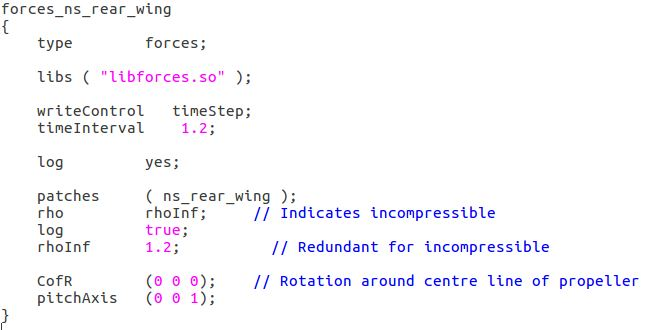
\includegraphics[width=9cm]{img/forces}
\caption{A part of code of forces file}
\end{center}
\end{figure}

The forces are collected from all car's patches. In result OpenFoam create file with forces and moments in all directions.


\subsection{Convert mesh to polyhedral}
Instead of tetrahedral mesh will be used polyhedral mesh, which has less elements, and calculations are more stable. From 15mln elements it was made 3mln. 

polyDualMesh is using to convert mesh to polyhedral. There is one argument - minimum angle between normals to cell's faces. In this calculation it is 30 degrees. Also it should be used options: -overwrite and -doNotPreserveFaceZones. First one (optional), overwrite new mesh in time 0, which is  comfortable. Second delete old faces from mesh. It is necessarily to correct work.

\begin{figure}[h!]
	\centering
    \begin{subfigure}[b]{0.46\linewidth}
    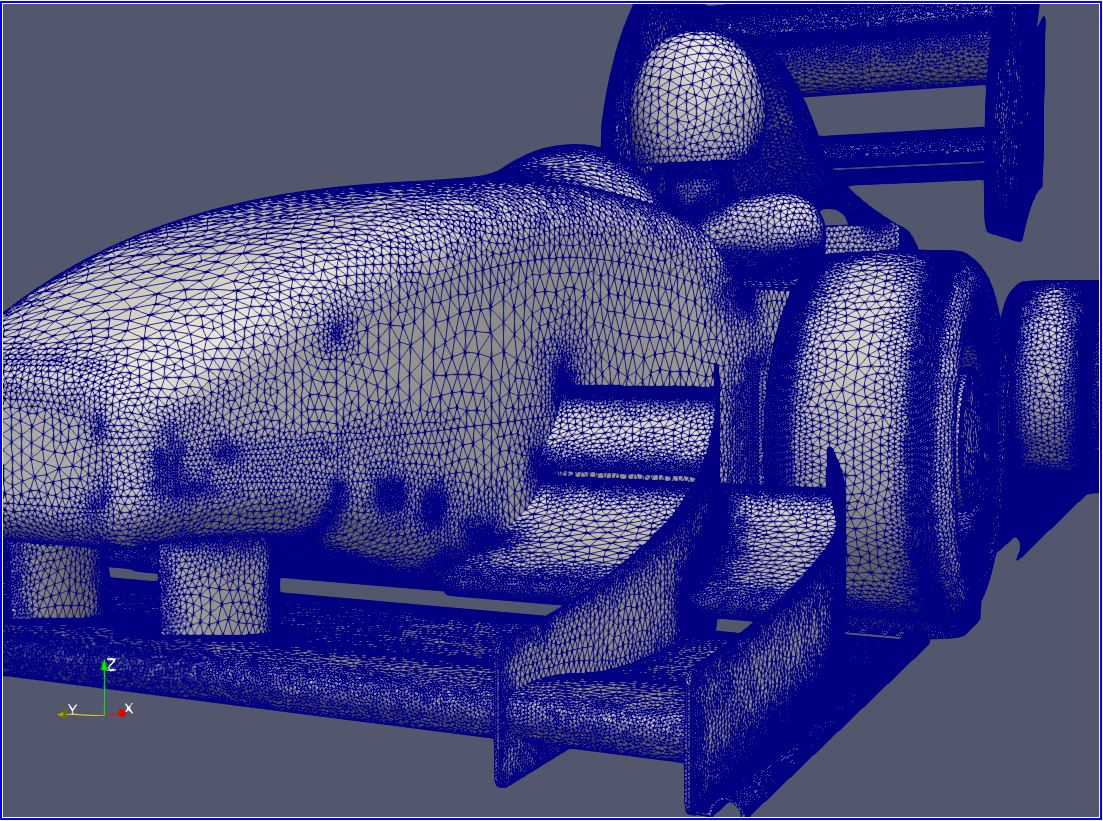
\includegraphics[width=\textwidth]{tetra.JPG}
    \caption{Tetrahedral mesh}
    \end{subfigure}
    
    \begin{subfigure}[b]{0.46\textwidth}
    	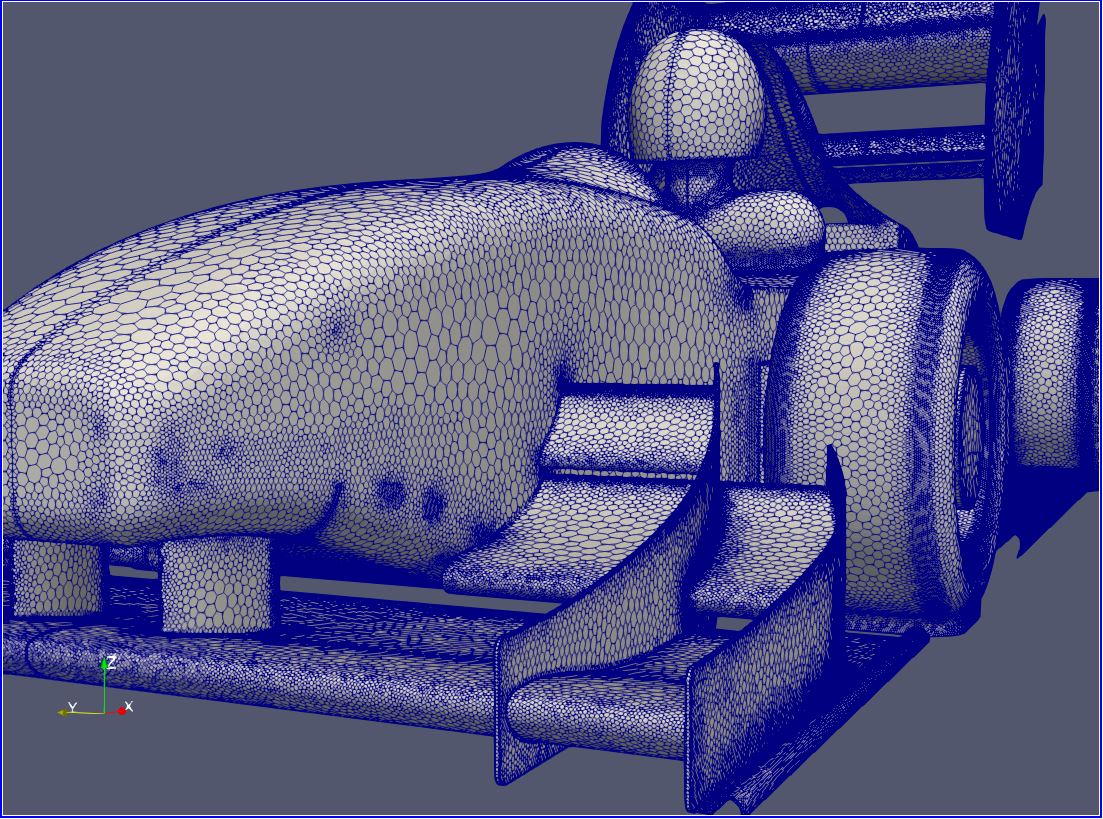
\includegraphics[width=\textwidth]{polyhedra.JPG}
        \caption{Polyhedral mesh}
    \end{subfigure}
    \begin{subfigure}[b]{0.46\textwidth}
    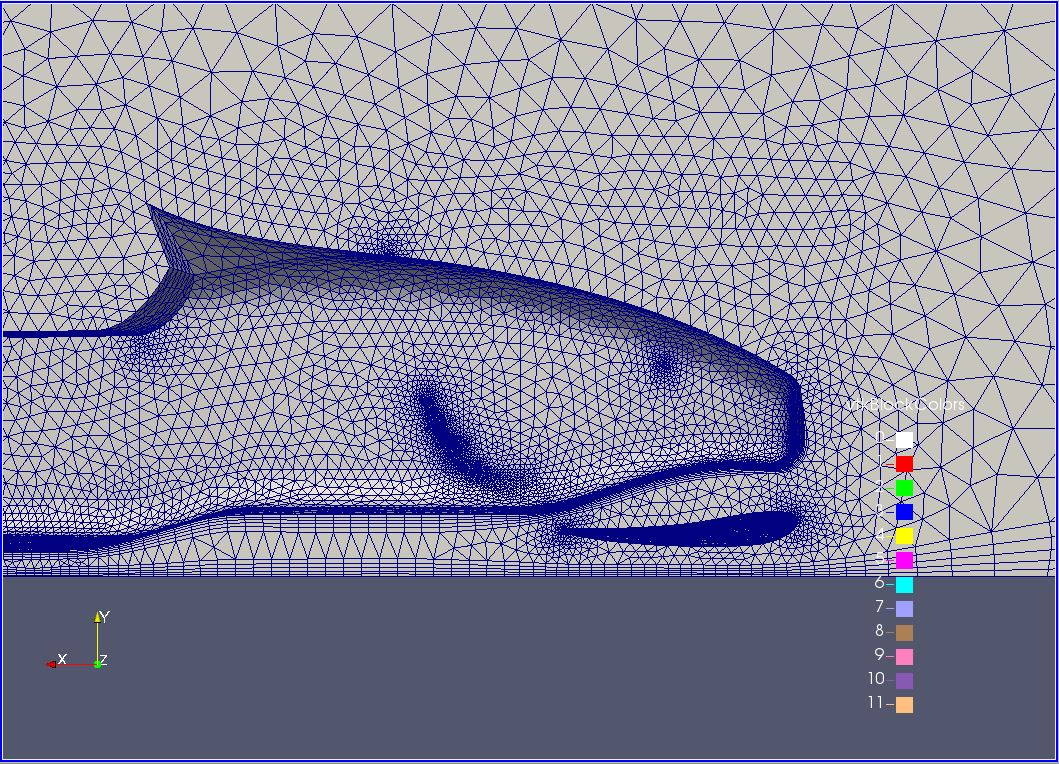
\includegraphics[width=\textwidth]{tetra2.JPG}
    \caption{Tetrahedral mesh}
    \end{subfigure}
    \begin{subfigure}[b]{0.46\textwidth}
    	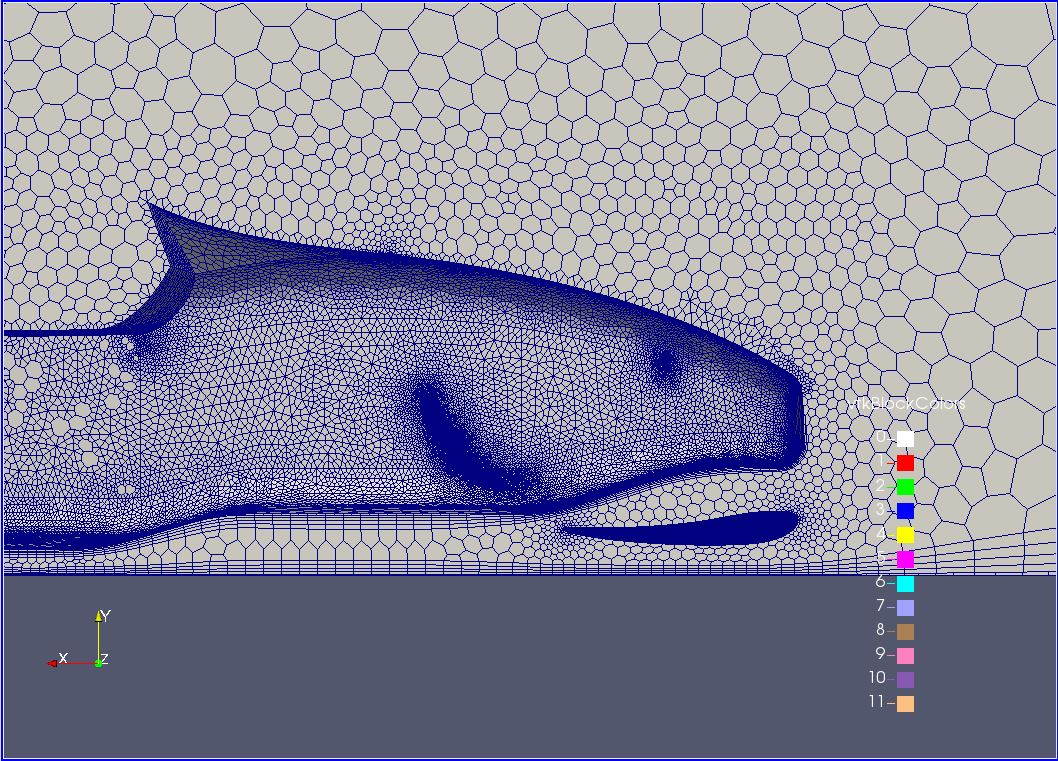
\includegraphics[width=\textwidth]{polyhedra2.JPG}
        \caption{Polyhedral mesh}
    \end{subfigure}
    \caption{Comparison both tetrahedral and polyhedral meshes}
\end{figure}


\subsection{Parallel calculations}
Calculation was carried out on 32 cores, on four EC2 instances. The instances have been merged to cluster. Scotch decompose method has been chosen. 

\subsection{Calculations}
There was 360 time steps and it was enough to stabilize forces and getting good accuracy.
\input{chapters/awscli}
\section{Create an OpenFoam cluster on AWS}

Large calculations require a lot of RAM memory and processor's cores. Without required memory the calculations cannot be carried out. With a small number of processors it woulde take a lot time. Sometimes, a signle instance is insufficient to make for example CFD calculations. It is possible to merge a few istances to make a larger one.

Create the OpenFoam cluster will be presented. The bash script has been created to automate calculations.

\subsection{Ssh Agent}

A premission master instance to slave instances is given by publikey (.pem) through ssh agent. To enable connect to instances without -i parameter, this script should be run:

\begin{figure}[h!]
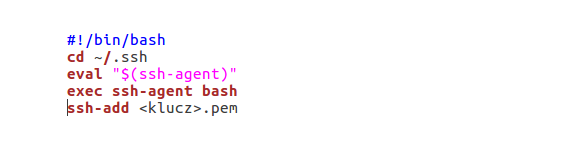
\includegraphics[width=\textwidth]{img/ssh_agent}
\caption{SSH Agent script}
%\label{fig:boat1}
\end{figure}

Lines begin with "eval" and "exec" are necesserly when something is going wrong.

\subsection{Sharing the Master Instance Volume}

Next script share the master instance volume to slave instances. All data is storage in master instance, slave instances share memory and processors' cores, but all data are save in master instance.

\begin{figure}[h!]
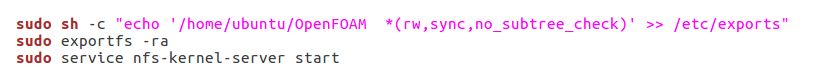
\includegraphics[width=\textwidth]{img/share_volume}
\caption{Share volume script}
%\label{fig:boat1}
\end{figure}

\subsection{Mounting the Master Volume from Slaves}

Next
\section{Results}
\subsection{Contours}
Images show contours of pressure and velocity around the car. It is able to see high pressure on the top of aerodynamic elements and negative pressure - under the elements. This difference generate down force which is useful in turns.
\begin{figure}[h!]
	\centering
    \begin{subfigure}[b]{0.48\textwidth}
    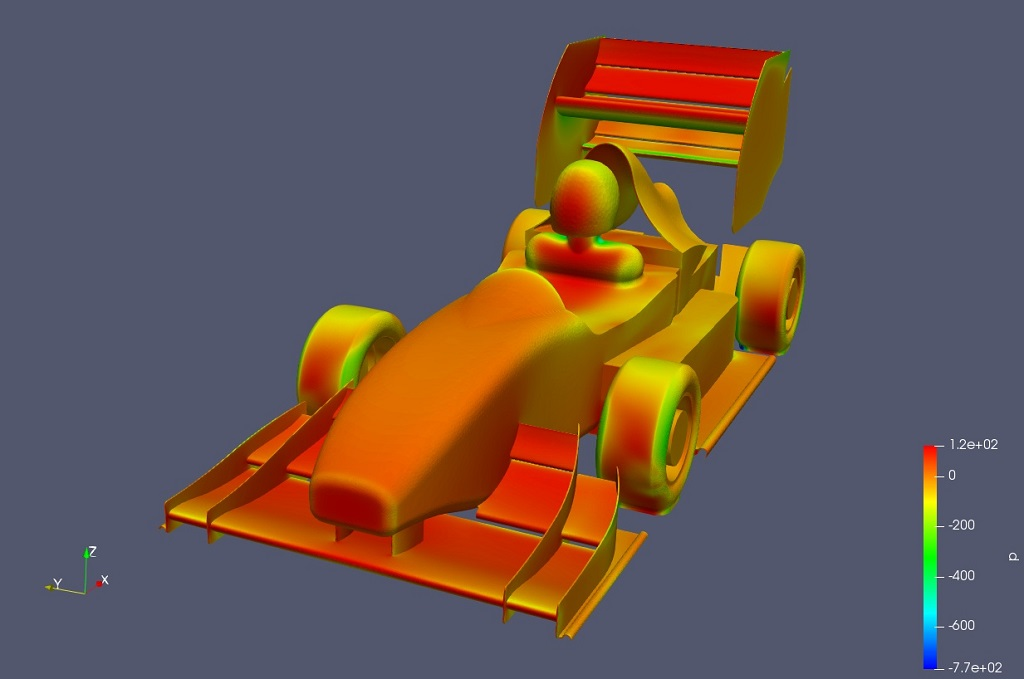
\includegraphics[width=\textwidth]{cis.jpg}
    %\caption{Pressure}
    \end{subfigure}
    \begin{subfigure}[b]{0.48\textwidth}
    	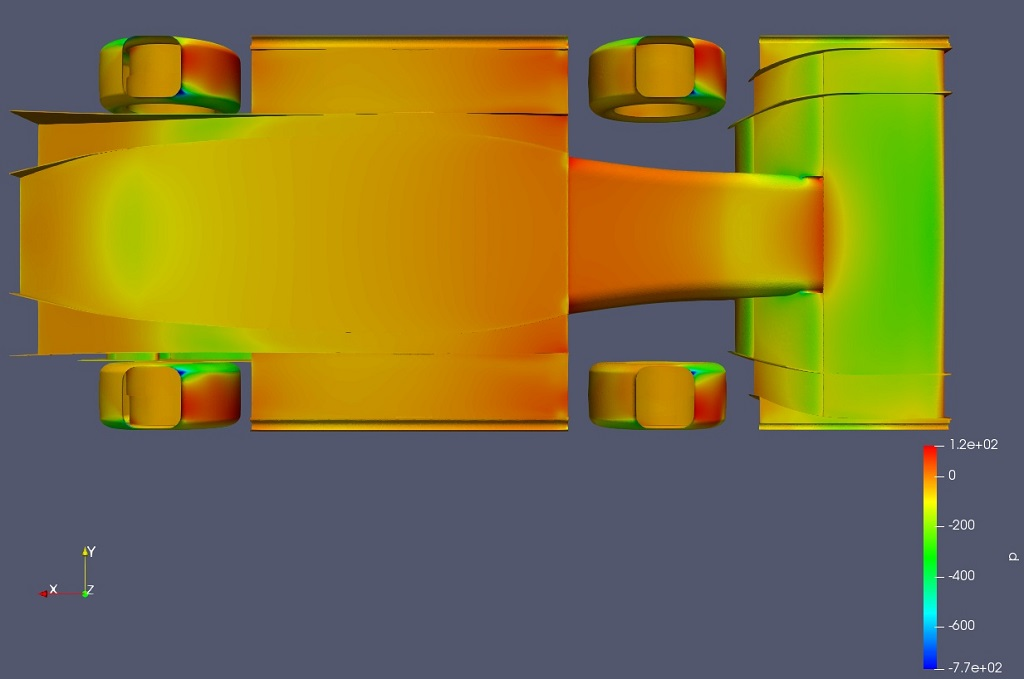
\includegraphics[width=\textwidth]{cis2.jpg}
        %\caption{Pressure}
    \end{subfigure}
    \begin{subfigure}[b]{0.48\textwidth}
    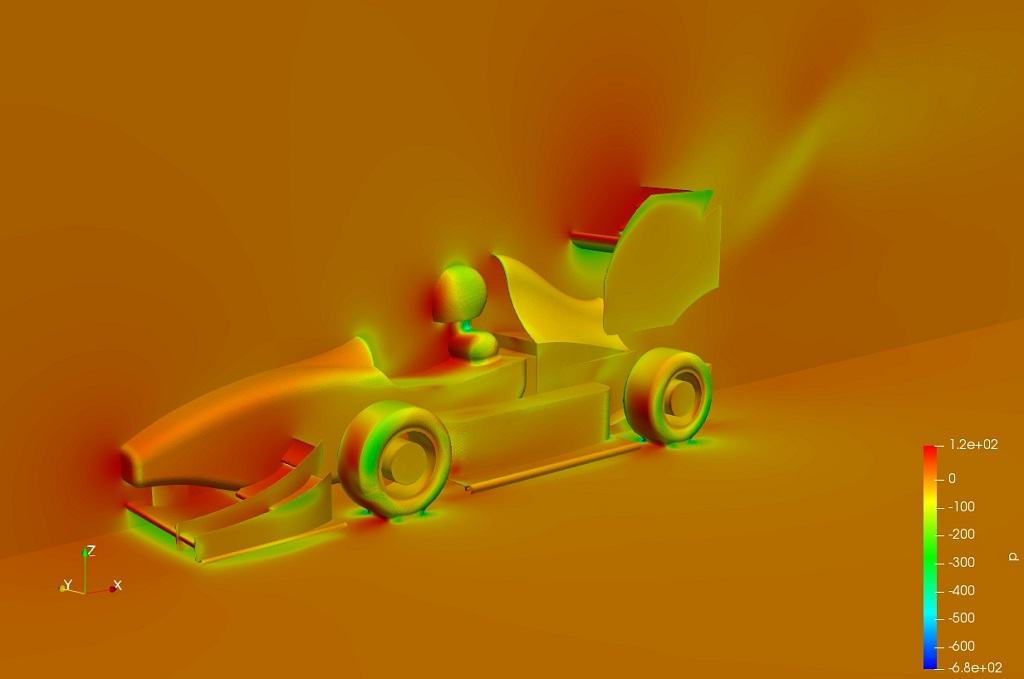
\includegraphics[width=\textwidth]{cis3.jpg}
    %\caption{Pressure}
    \end{subfigure}
    \begin{subfigure}[b]{0.48\textwidth}
    	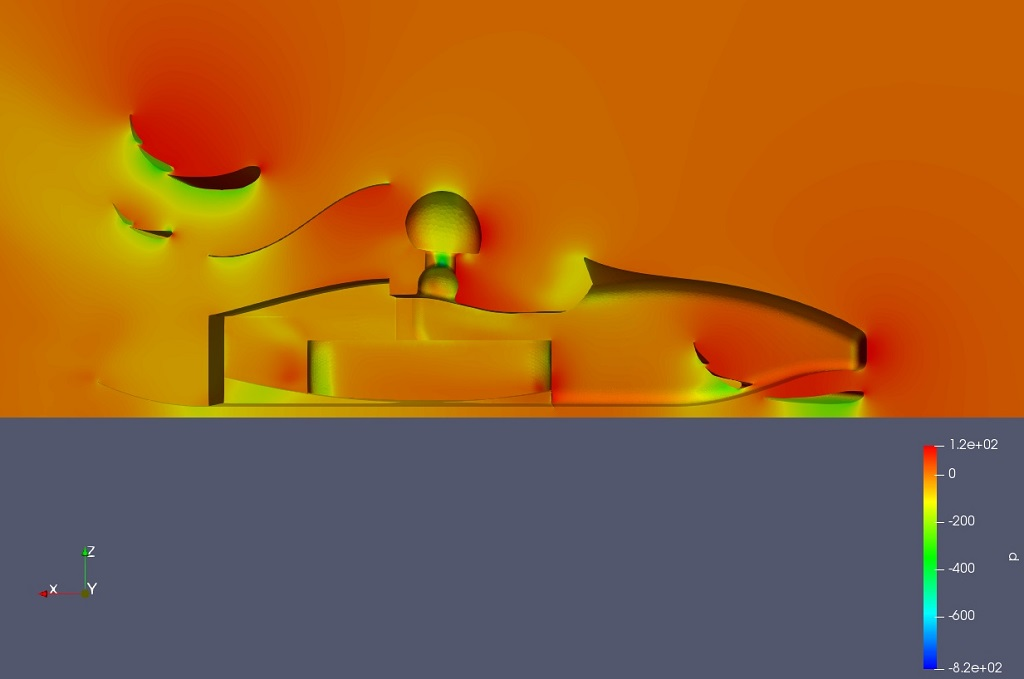
\includegraphics[width=\textwidth]{cis_sym.jpg}
        %\caption{Pressure}
    \end{subfigure}
    \caption{Contours of pressure}
    \begin{subfigure}[b]{0.7\textwidth}
    \centering
    	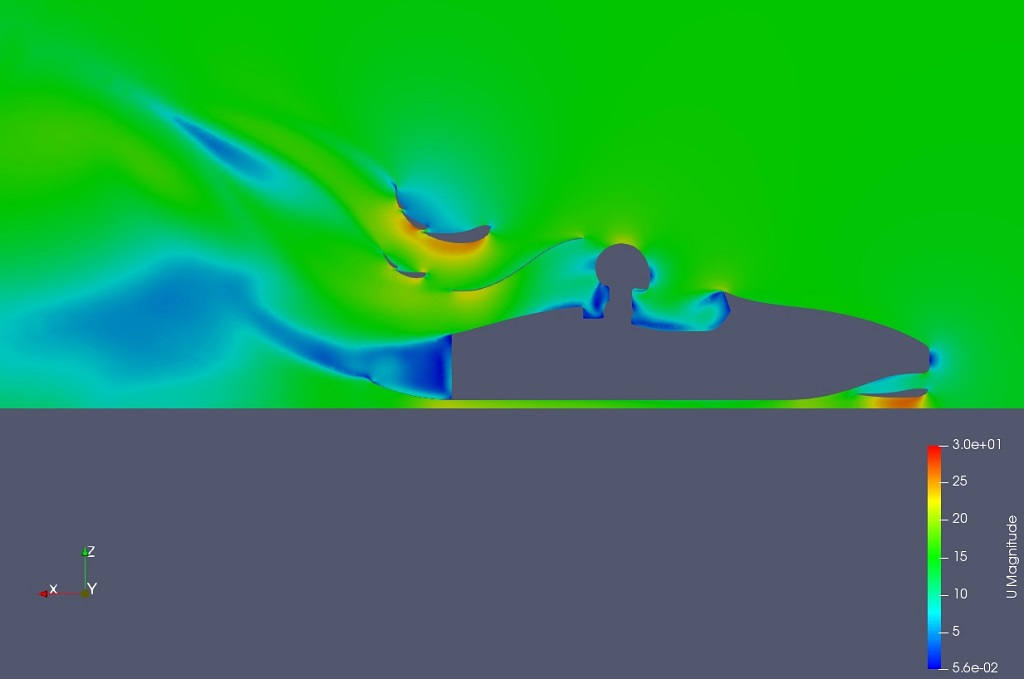
\includegraphics[width=0.7\textwidth]{vel.jpg}
    \end{subfigure}
    \caption{Contours of velocity}
\end{figure}

\newpage
Good visualization of the flow are streamlines which show, how air flow over (and under) the car. They give many information and they help improving the construction. 
\begin{figure}[h!]
	\centering
    \begin{subfigure}[b]{0.49\textwidth}
    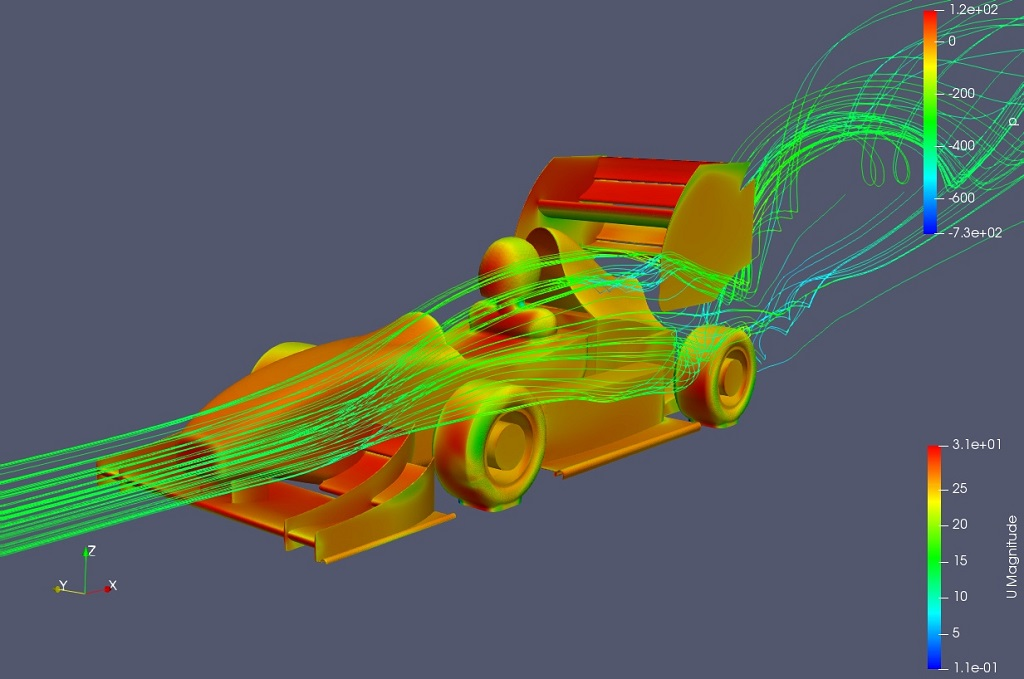
\includegraphics[width=\textwidth]{linie.jpg}
    %\caption{}
    \end{subfigure}
    \begin{subfigure}[b]{0.49\textwidth}
    	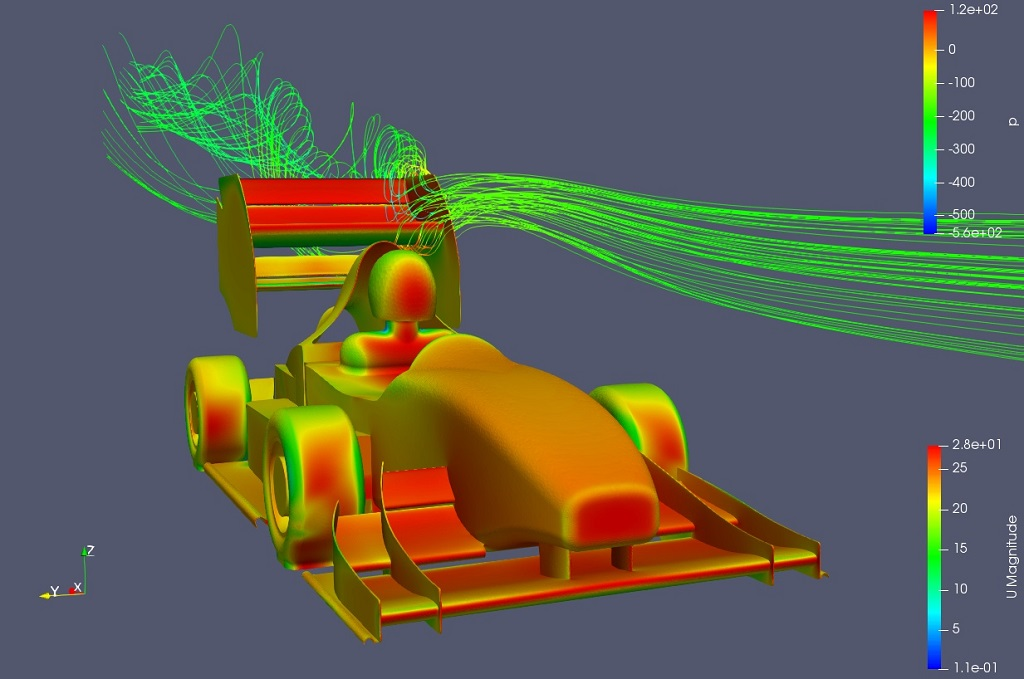
\includegraphics[width=\textwidth]{linie2.jpg}
        %\caption{}
    \end{subfigure}
    \begin{subfigure}[b]{0.49\textwidth}
    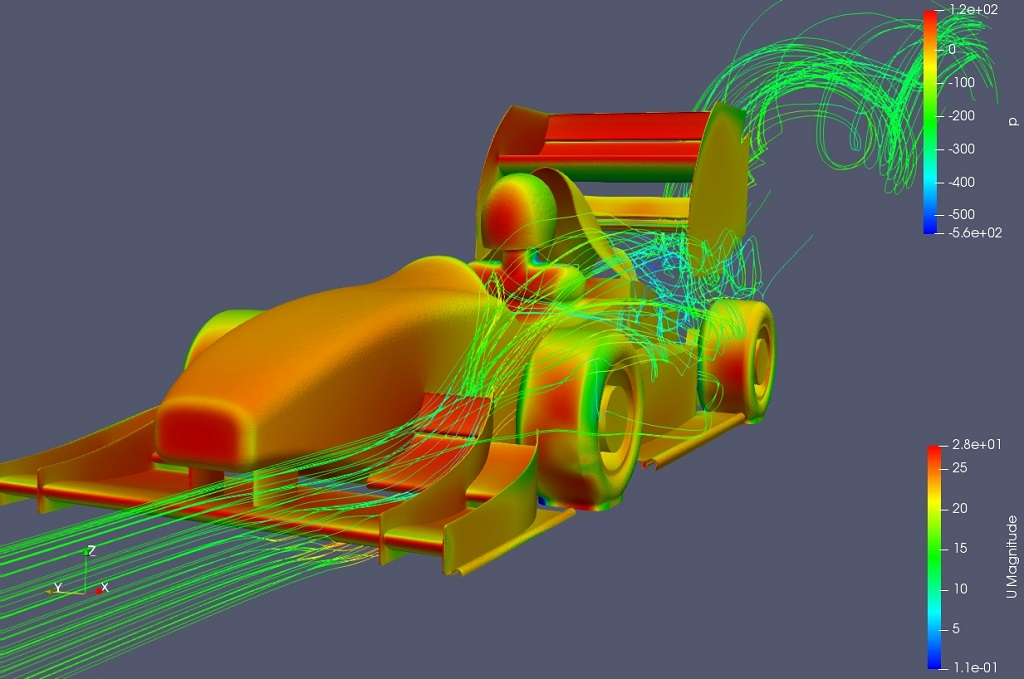
\includegraphics[width=\textwidth]{linie3.jpg}
    %\caption{}
    \end{subfigure}
    \begin{subfigure}[b]{0.49\textwidth}
    	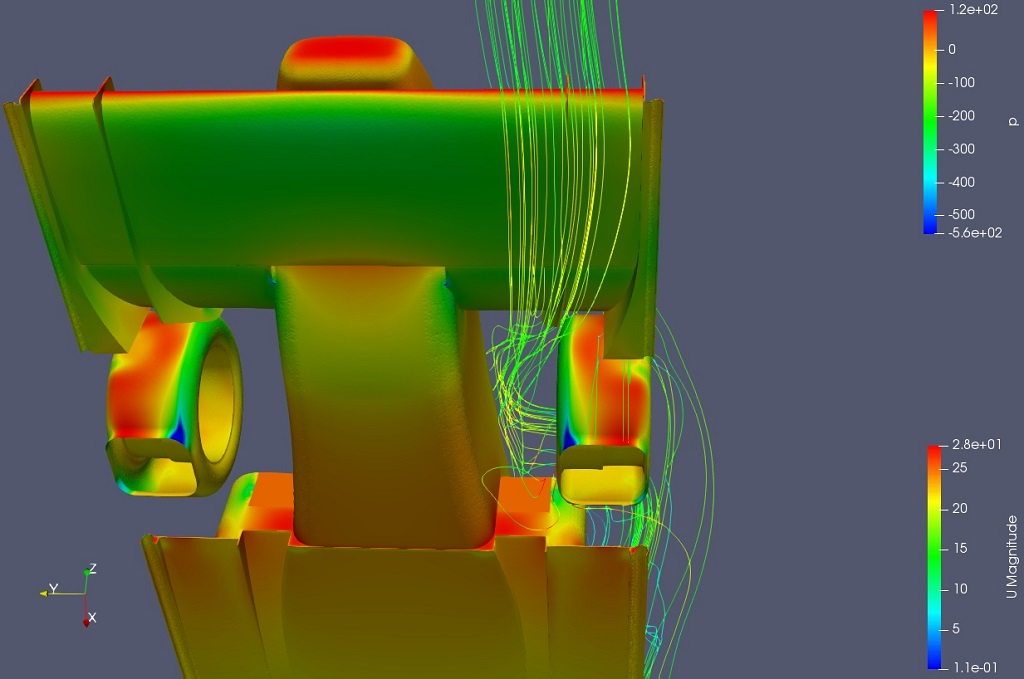
\includegraphics[width=\textwidth]{linie4.jpg}
        %\caption{}
    \end{subfigure}
    \caption{Streamlines}
   
\end{figure}


\subsection{Comparison with Fluent}
The same calculation has been carried out in Fluent, one of the best CFD software. Is OpenFoam, as open source, free software, as good as commercial software? The down forces and coefficients will be compared:

\begin{tabular}{lr|c|c}
Patch		&	OpenFoam		&	Fluent		&Difference\\\hline
Rear Wing	&-178N				&-186N			&4\%\\
Front Wing	&-132N				&-156N			&15\%\\
Diffuser	&-112N				&-98N			&-14\%\\
Others		&92N				&102N			&-10\%\\\hline
Sum			&-330N				&-338N			&2\%\\\hline\hline
Cl			&-2,11				&-1,9			&-11\%\\
Cx			&0,87				&0,95			&-8\%\\

\end{tabular}

Differences are about 10\% between OpenFoam and Fluent. It is quite a lot. The reason may be in low mesh quality and not enough elements. 
\input{chapters/summarise}








\newpage
\rhead{
\includegraphics[height=1.5cm]{AmazonS3.png}}
\section{Working on AWS Amazon}

The case has been create on PC and coarse mesh has been converted to OpenFoam format to check entire case. When the case was correct, it has been sent to S3 storage with fine mesh. 

EC2 instances was launched as Spot Request Instance, because of the lower price (about 70\% in compare to On Demand Instances). Then the files was download from S3 to EC2 instance by command "aws s3 cp s3://bucket-name/file ./". Next it has been working as in normal PC. 

The results has been sent to S3 by command "aws s3 sync <folder> s3://bucket-name/folder" or it was download directly by FileZilla to PC.

\section{Summarize}
The OpenFoam is very good free software, but in more complex calculations it might fail. I think that in better mesh, difference between OpenFoam and Fluent could be smaller. However, Fluent's solver is more stable (calculate low quality meshes), but very expensive. In the near future, calculations will be validated in aerodynamic tunnel in our faculty.





\end{document}